\documentclass[11pt]{article}

\usepackage{fullpage}
\usepackage{amsmath}
\usepackage{amssymb}
\usepackage{amsthm}
\usepackage{fancyhdr}
\usepackage{algorithm}
\usepackage{algorithmic}
\usepackage{bm}
\usepackage{listings}
\usepackage{graphicx}
\usepackage{caption2}
\usepackage{subfigure}
\usepackage{float}
\usepackage{extpfeil}
\usepackage{color}
\usepackage[usenames,dvipsnames]{xcolor}


\newtheorem{theorem}{Theorem}[section]
\newtheorem{lemma}[theorem]{Lemma}
\newtheorem{corollary}[theorem]{Corollary}
\newtheorem{proposition}[theorem]{Proposition}
\newtheorem{definition}[theorem]{Definition}
\newtheorem{conjecture}[theorem]{Conjecture}
\newtheorem{remark}[subsection]{Remark}

%%
\newcommand\numberthis{\addtocounter{equation}{1}\tag{\theequation}}

%% define new symbols
\def\bx{\bm{x}}
\def\bb{\bm{b}}
\def\ba{\bm{a}}
\def\bc{\bm{c}}
\def\bf{\bm{f}}
\def\by{\bm{y}}
\def\bu{\bm{u}}
\def\bv{\bm{v}}
\def\BW{\bm{W}}
\def\BA{\bm{A}}
\def\bz{\bm{z}}
\def\BZ{\bm{Z}}
\def\BH{\bm{H}}
\def\BL{\bm{L}}
\def\BU{\bm{U}}
\def\BV{\bm{V}}
\def\BB{\bm{B}}
\def\BC{\bm{C}}
\def\BD{\bm{D}}
\def\BE{\bm{E}}
\def\BW{\bm{W}}
\def\BQ{\bm{Q}}
\def\BG{\bm{G}}
\def\BA{\bm{A}}
\def\BX{\bm{X}}
\def\BY{\bm{Y}}
\def\BQ{\bm{Q}}
\def\BI{\bm{I}}
\def\BR{\bm{R}}

%% define new brackets
\def\la{\left\langle}
\def\ra{\right\rangle}
\def\ln{\left\|}
\def\rn{\right\|}
\def\lb{\left(}
\def\rb{\right)}
\def\lsb{\left[}
\def\rsb{\right]}
\def\lcb{\left\{}
\def\rcb{\right\}}

%%
\DeclareMathOperator*{\argmin}{arg\,min}
\DeclareMathOperator*{\argmax}{arg\,max}

%%
\title{Homework II}
\author{Name: Shao Yanjun, Number: 19307110036}


\begin{document}
\maketitle

%------------------------------------
\begin{abstract}
This is Daniel's homework of  "Numerical Algorithms with Case Studies II".
\end{abstract}
%-------------------------------------
%=====================
\section{Problems}
\paragraph{Q1}
We first observe the figure of $f(x)=\arctan(x)$, and make a few guesses that the intersection of the tangent at $\alpha$ with the axis coincidentally falls on $-\alpha$. I will give out the direct equation to look for $\alpha$,
\begin{align}
	f(\alpha)=\arctan(\alpha)-\frac{2\alpha}{1+\alpha^2}=0
\end{align}
\hspace*{0.4cm}
Use Newton method, calculate the zero point of $f(\alpha)$ with Matlab. $\alpha\approx1.3917452002$
\begin{figure}[H]
	\centering
	\subfigure[arctan(x)]{
		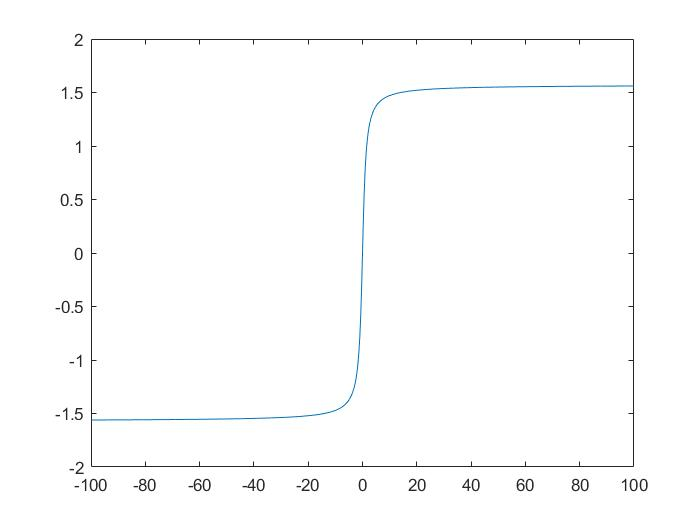
\includegraphics[width=0.4\linewidth]{arctan.jpg}
	}
	\subfigure[Newton method fails]{
		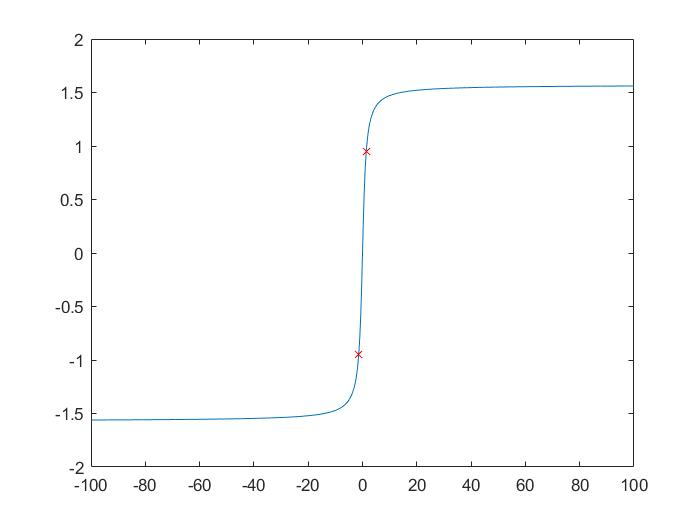
\includegraphics[width=0.4\linewidth]{H2Q1.jpg}
	}
\end{figure}
After this, conduct Newton method for $\arctan(x)$ with the initial guess. The result is upset, since we couldn't get to the zero point. Instead, the $x$ is always skipping from $\alpha$ to $-\alpha$.
\paragraph{Q2}
The solution with method bisection gives $x_1=0.964661619910657$, while the other gives $x_2=0.964661619911055$. Basically, $x_1$ and $x_2$ are identifical with accuracy of $10^{-11}$.\\
Here are the convergence analysis and searching procedure of bisection method and regula falsi method.
\begin{figure}[H]
	\centering
	\subfigure[bisection]{
		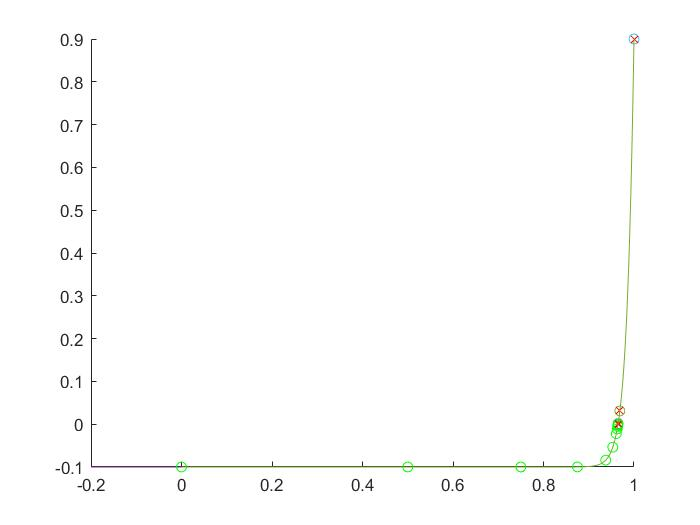
\includegraphics[width=0.4\linewidth]{bisection.jpg}
	}
	\subfigure[convergence]{
		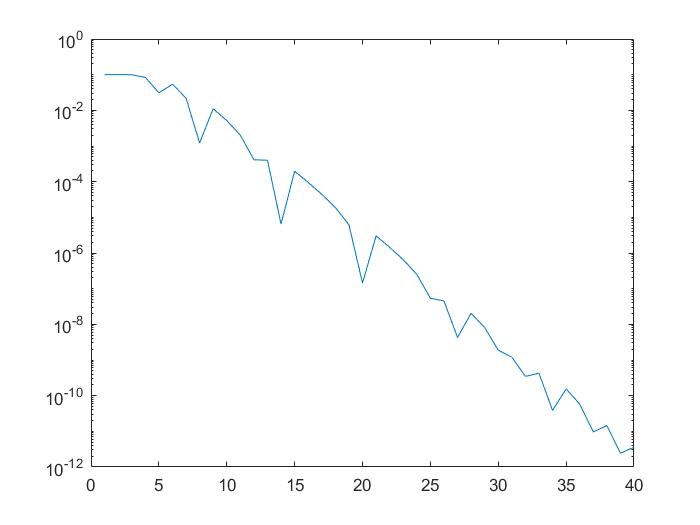
\includegraphics[width=0.4\linewidth]{bisection_loss.jpg}
	}
\centering
\subfigure[regula falsi]{
	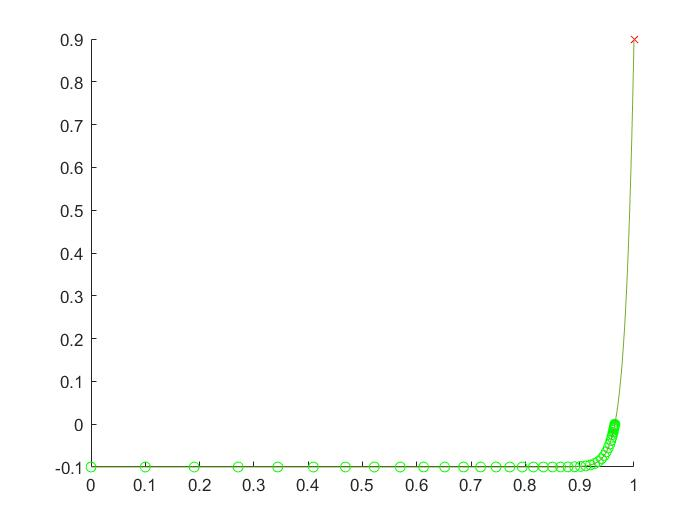
\includegraphics[width=0.4\linewidth]{regula_falsi.jpg}
}
\subfigure[convergence]{
	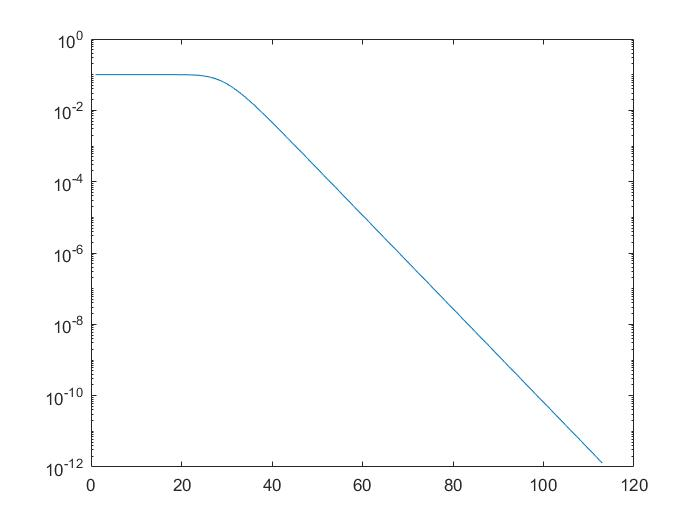
\includegraphics[width=0.4\linewidth]{regula_falsi_loss.jpg}
}
\end{figure}
Note that both loss function are output in semilogy(). And bisection method converges far better than regula falsi in this case.
\paragraph{Q3}
Here is the $x=f(y)$ and $y=f^{-1}(x)$ plot in one figure. And they perfectly match with each other if we fold across $y=x$.
\begin{figure}[H]
	\centering
	\subfigure[$x=ye^y$ and $y=lambertW(x)$]{
		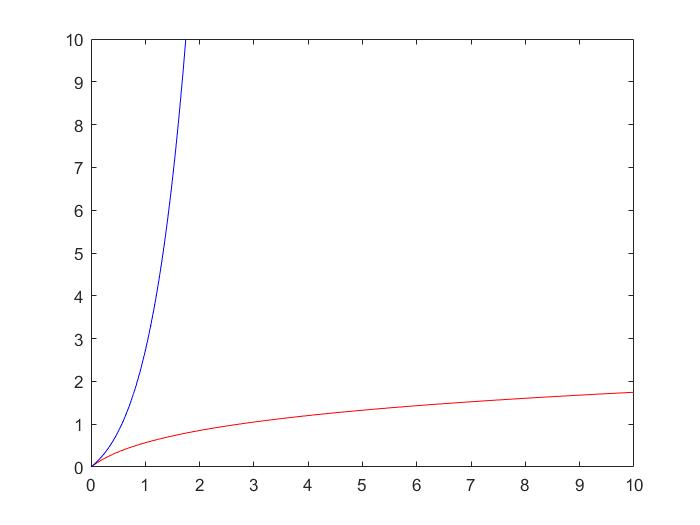
\includegraphics[width=0.4\linewidth]{H2Q3_1.jpg}
	}
	\subfigure[match after folding]{
		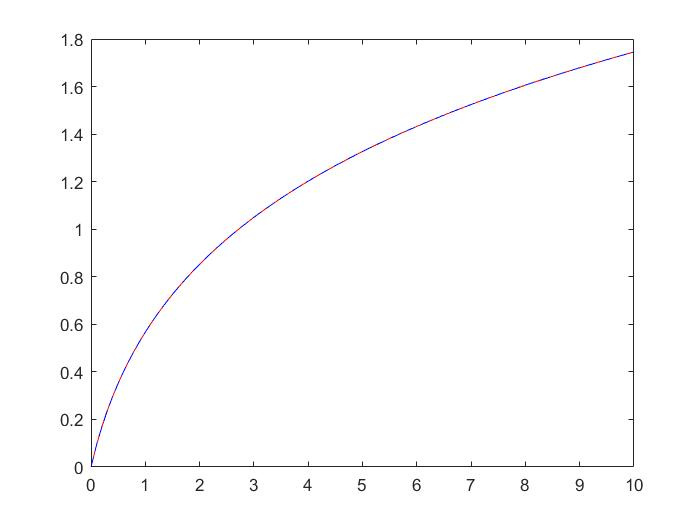
\includegraphics[width=0.4\linewidth]{H2Q3_2.jpg}
	}
\end{figure}
\paragraph{Q4}
\subparagraph{(a)}
The solution is $x=3.141591575732336$, which is not exactly $\pi$ because of the truncating error.
\begin{figure}[H]
	\centering
	\subfigure[Newton loss]{
		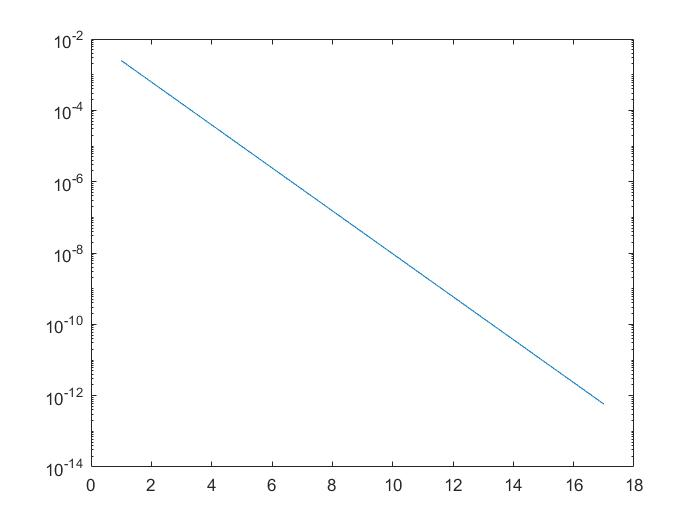
\includegraphics[width=0.5\linewidth]{Newton_loss.jpg}
	}
\end{figure}
Through observation, we conclude that Newton method is linearly convergent in this case.
\subparagraph{(b)}
Use the Newton iteration formula $x_{k+1}=x_{k}-\frac{f(x_k)}{f'(x_k)}$, and the Taylor expansion $f(x_k)=f(x_*)+f'(x_*)(x_k-x_*)+\frac{1}{2!}f''(\xi)(x_k-x_*)^2, (x_k<\xi<x_*)$. As $f(x_*)=0$ and $f'(x_*)=0$, we could get an estimation of convergence,
\begin{align}
	\|x_{k+1}-x_*\|&=\|x_k-x_*-\frac{f'(\eta)}{2f'(\xi)}(x_k-x_*)\|,\quad (x_k<\eta<x_*\quad and \quad x_k<\xi<x_* ) \\
	&=|1-\frac{f'(\eta)}{2f'(\xi)}|\|x_k-x_*\|\le C\|x_k-x_*\|
\end{align}
This exhibits linear convergence.
\subparagraph{(c)}
Similarly, we apply a further Taylor expansion $f(x_k)=f(x_*)+f'(x_*)(x_k-x_*)+\cdots+\frac{1}{(m+1)!}f^{(m+1)}(\xi)(x_k-x_*)^{m+1}, (x_k<\xi<x_*)$. With the modified method $x_{k+1}=x_k-\frac{(m+1)f(x_k)}{f'(x_k)}$ and the given property $f'(x_*)=\cdots=f^{(m)}(x)=0\ne f^{(m+1)}(x)$, we could get an estimation of convergence as below,
\begin{align}
	\|x_{k+1}-x_*\|&=\|x_k-x_*-\frac{f^{(m+1)}(\eta)}{f^{(m+1)}(\xi)}(x_k-x_*)\|,\quad (x_k<\eta<x_*\quad and \quad x_k<\xi<x_* ) \\
	&=|1-\frac{f^{(m+1)}(\eta)}{f^{(m+1)}(\xi)}|\|x_k-x_*\|
	=\frac{|f^{(m+1)}(\xi)-f^{(m+1)}(\eta)|}{|f^{(m+1)}(\xi)|}\|x_k-x_*\|\\
	&=\frac{|f^{(m+2)}(\tau)|}{|f^{(m+1)}(\xi)|}\|\eta-\xi\|\|x_k-x_*\|,\quad (\xi<\tau<\eta)\\
	&\le \frac{|f^{(m+2)}(\tau)|}{|f^{(m+1)}(\xi)|}\|x_k-x_*\|^2
\end{align}
This exhibits quadratic convergence.
%-------------------------------------
%=====================
\end{document}
